\documentclass[12pt, a4paper, twoside]{article}

%% Preamble
\usepackage{pdfpages}           % Para incluir PDFs
\usepackage{graphicx}           % Para gráficos
\usepackage{subfiles}           % Para manejar subarchivos
\usepackage{hyperref}           % Para enlaces
\usepackage{listings}           % Para código fuente (ajusta lenguaje)
\usepackage{verbatim}
\usepackage[backend=bibtex,style=numeric]{biblatex} % Para citas numéricas
\addbibresource{references.bib} % Cargar archivo .bib
\usepackage{url}


\usepackage{geometry}           % Para ajustar márgenes

% Ajustes de márgenes
\geometry{
	left=3cm,       % Margen izquierdo
	right=3cm,      % Margen derecho
	top=2.5cm,      % Margen superior
	bottom=2.5cm,   % Margen inferior
	headheight=15pt, % Altura del encabezado
	twoside          % Para documentos a dos caras
}


\graphicspath{{images/}{../images/}} % Ruta para imágenes

\begin{document}
	
	%% Cover
	
\includepdf[noautoscale=true, width=\paperwidth]{cover.pdf}
	
	%% Title
	\clearpage
	\setcounter{page}{1}
	
\includepdf[noautoscale=true, width=\paperwidth]{title.pdf}
	
	%%%%%%%%%%%%%%%%%%%%%%%%%%%%%%%%%%%%%%%%%%%%%%%%%%%%%%%%%%%%%%%%%%%%%%%%%%%
	
	% Índice automático
	\tableofcontents
	\newpage
	
	% Sections
	
		% Sections
	\section{Introducción}
	
	\section{Diario de avances}
	
	\subsection{Registro 3-16 de marzo)}
	
	Por ahora lo que llevamos es un dataset hecho en roboflow con un partido de España contra Suiza. Realizamos capturas y dividimos el conjunto en training, validation y test.
	
	Entrené el modelo de YOLO con este dataset revisado y el modelo no supo detectar bien el balón debido a la poca cantidad de imágenes donde se pueda ver bien la bola. El árbitro y los jugadores fueron bien detectados.
	
	Se replanteó el objetivo del TFG. Se focalizará en la reidentificación de jugadores cuando salen fuera de plano y en el desarrollo de una aplicación que permita al usuario decidir si cuando se produce un cambio de identificador, mantenerlo o cambiarlo, creando un dataset revisado.
	
	\subsection{Registro 17 marzo}
	
	A la hora de medir resultados como estas gráficas:
	
	\begin{figure}[h]
		\centering
		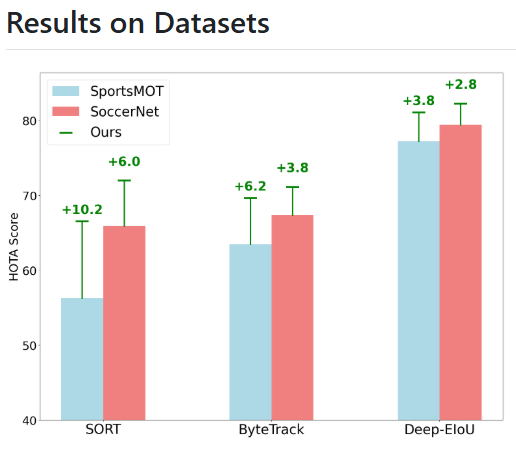
\includegraphics[width=0.8\textwidth]{image/metricasBeta}
		\caption{\textbf{Métricas gta\_link}}
		\label{fig:metricasBeta}
	\end{figure}
	
	Nos centraremos en la medida de los ID's intentando minimizarlos, lo máximo posible, ya que la métrica significa número de ids generados.
	
	\begin{figure}[h]
		\centering
		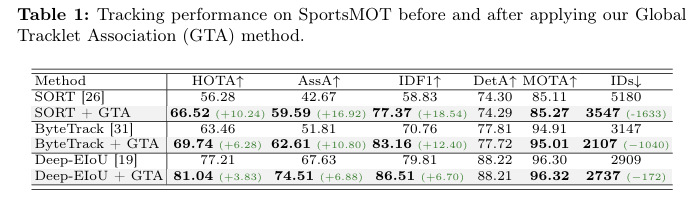
\includegraphics[width=0.8\textwidth]{image/Centrarse}
		\caption{\textbf{Objetivo}}
		\label{fig:Centrarse}
	\end{figure}
	
	
	
	
	%%%%%%%%%%%%%%%%%%%%%%%%%%%%%%%%%%%%%%%%%%%%%%%%%%%%%%%%%%%%%%%%%%%%%%%%%%%
	\printbibliography
	
	
	%% Back Cover
	
\includepdf[noautoscale=true, width=\paperwidth]{backcover.pdf}
	
\end{document}